\documentclass{book}
\usepackage[english]{babel}
\usepackage[letterpaper,top=2cm,bottom=2cm,left=3cm,right=3cm,marginparwidth=1.75cm]{geometry}

\usepackage{amsmath}
\usepackage{graphicx}
\usepackage[export]{adjustbox}

\usepackage[colorlinks=true, allcolors=blue]{hyperref}

\title{Molecular Pharmacology Notes}
\author{Elisa Pettinà}

\begin{document}
\maketitle

\chapter{Introduction: PK/PD}
\section{{What is a drug?}}
\textbf{A drug is a chemical that interacts with proteins in the body to affect a physiological function}.
Once these chemicals are absorbed into the systemic circulation they bind with certain proteins and this changes the functioning of the cell slightly. 
For example, anticancer drugs bind to proteins on the surface of cancer cells this stimulates the cells to die. 
In this case cell death is the physiological action of the drug.
\\
No drugs are specific to interacting with just one type of cell or one type of protein
and this is what causes \textbf{side effects}. 
Again using an anticancer drug as an example, the medication works by binding to very rapidly dividing cells, such as cancer cells, however hair cells are also rapidly dividing and that is why one of the side effects of anticancer drugs is hair loss.
\\
Drugs can be generally divided into two main categories: \textbf{agonist}, that stimulate a response and \textbf{antagonist}, that inhibit a response.

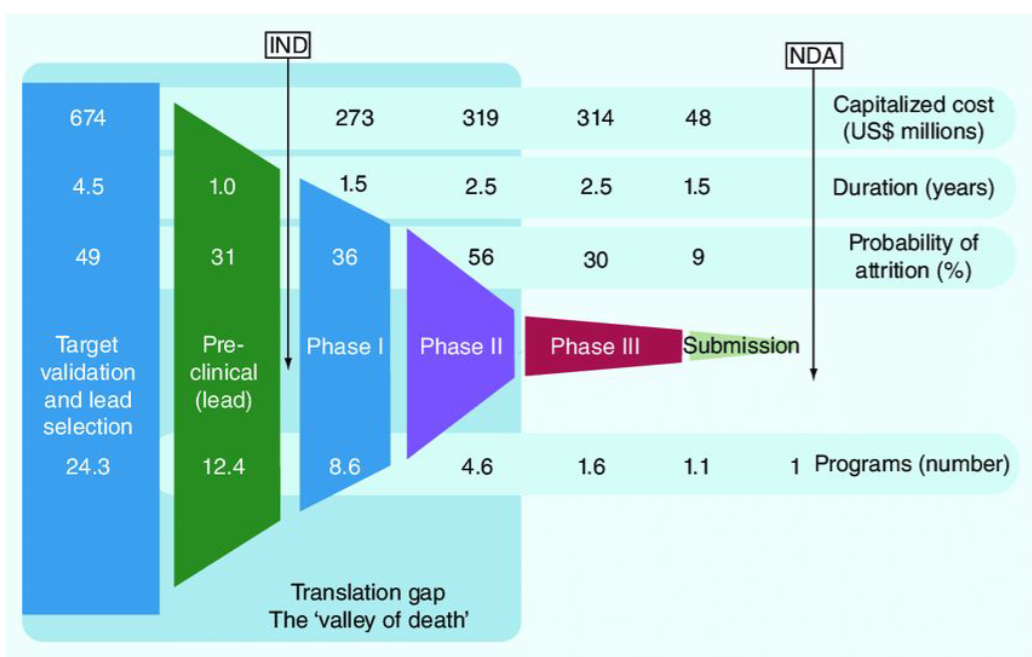
\includegraphics[width=0.7\textwidth, center]{images/image.png}

Developing and testing drugs is a very expensive business!
Many parameters regarding pharmacokinetics and pharmacodynamycs need to be taken studied and fit into strict boundaries for the drug to be accepted.

\section{Pharmacokinetics}
Pharmacokinetics (PK) is the study of how the body interacts with administered substances for
the entire duration of exposure.
In other words, \textbf{what the body does to the drug(s)}!
\\
For a chemical compound to become a marketable drug, it must have favourable properties in addition to \textbf{efficacy} (its therapeutic effect) and \textbf{safety}. 
These properties are summarised in the acronym ADME, which refers to \textbf{absorption}, \textbf{distribution}, \textbf{metabolism} and \textbf{excretion}.

\begin{itemize}
    \item Absorption: a compound's ability to pass through barriers such as the intestinal lining, the nasal lining, the lungs or the skin.
    \item Distribution: how the compound is distributed around the body and its propensity to accumulate in certain tissues and organs.
    \item Metabolism: how the body breaks down the compound, normally by the liver. The key issues are drug-drug interactions and the effects of the metabolites (the new chemicals created as a result of metabolism).
    \item Excretion: the rate and process through which the compund exits the body.
\end{itemize}

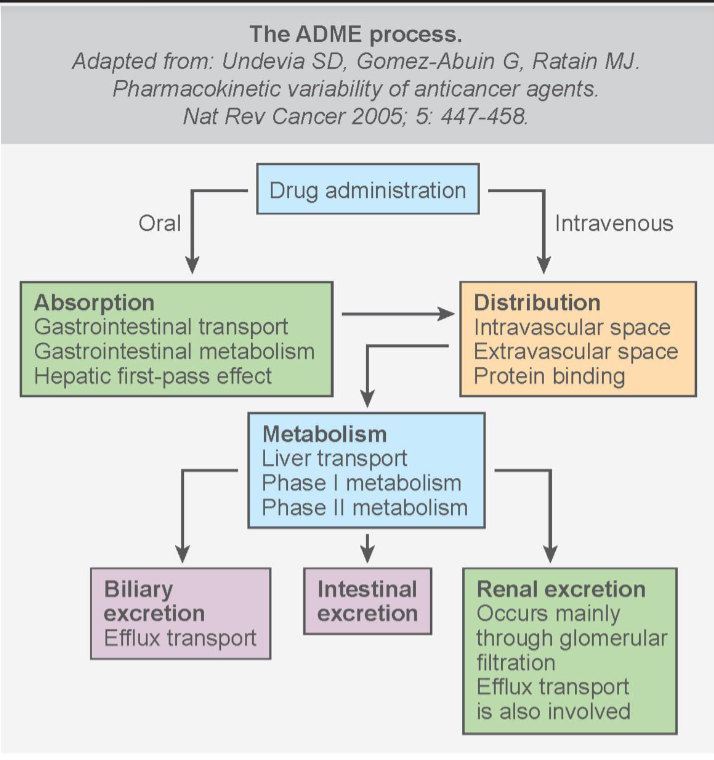
\includegraphics[width=0.6\textwidth, center]{images/image_1.png}

Often we refer also to \textbf{AADME}, including also \textbf{administration}, which also greatly influences the PK properties of drugs and drug concentration in plasma.

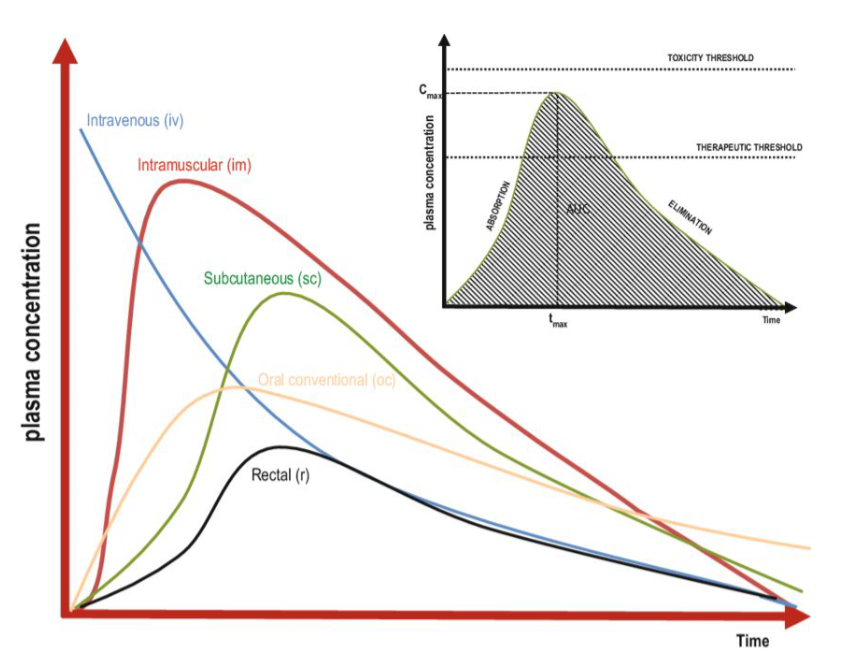
\includegraphics[width=0.6\textwidth, center]{images/image2.png}


\subsection{Absorption}
\textbf{Absorption is the process of a drug moving from its site of delivery into the bloodstream}.
\\
Absorption is the process of delivering a drug into the bloodstream. 
Absorption can be accomplished by administering the drug in a variety of different ways (e.g. orally, rectally, intramuscularly, subcutaneously, inhalation, topically, etc.). 
Note, that if a drug is administered intravenously (placed directly into the bloodstream), the need for absorption is bypassed entirely.
\\
However, the plasmatic membrane cannot be passed freely.
Gases ($CO_2$, $N_2$, $O_2$, anaesthetic), small uncharged polar molecules (ethanol, urea, water) can pass easily. Inversely, large uncharged polar molecules (sugar), ions and charged polar molecules (amino acids, ATP, proteins, nucleic acids) cannot.
\\
\\
The need for drug molecules to cross lipid bilayers in passing from one body compartment to another requires that the structure has properties that impart solubility in both a hydrophobic medium and water. 
Each part of a drug molecule contributes hydrophobic or hydrophilic properties to the molecule as a whole and that contribution is known as the \textbf{Hansch partition coefficient} of the
group.

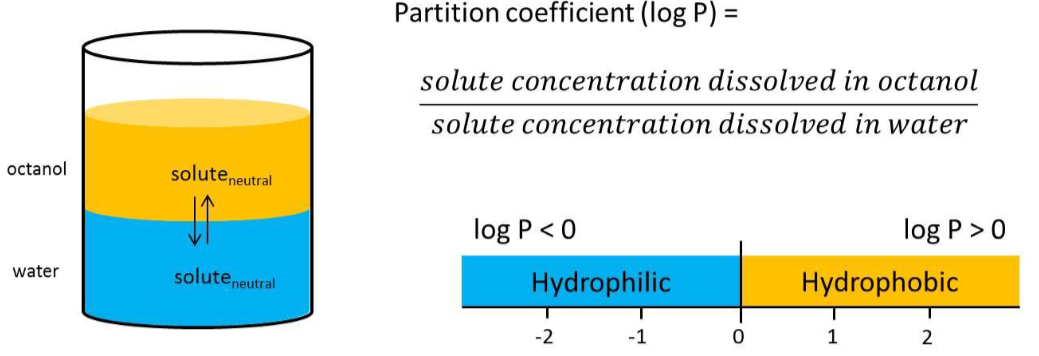
\includegraphics[width=0.6\textwidth, center]{images/image3.png}

\subsection{Distribution}
\textbf{Drug distribution is the process of delivering a drug from the bloodstream to
the body}.
The process of transferring a drug from the bloodstream to tissues is referred to as distribution. 
The same principles that govern drug absorption (e.g. ionization of a drug, lipophilicity of a drug, size of a drug, pH of the environment, etc.) also govern the rate and extent that a drug will distribute to various tissues in the body. 
In addition to that, there are additional factors at play, particularly non-specific binding to proteins.

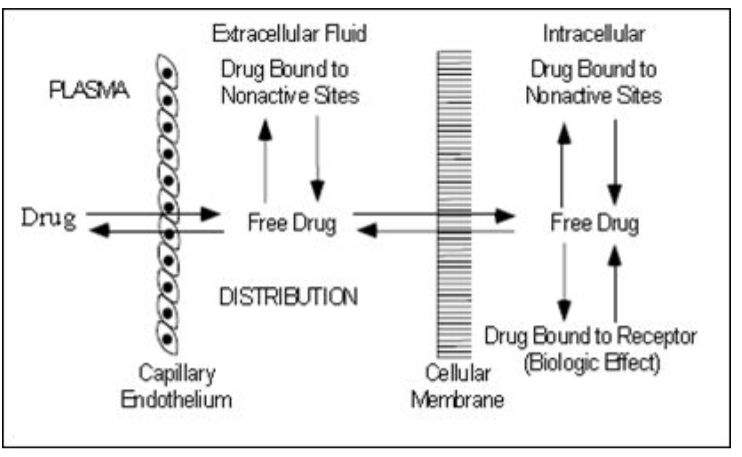
\includegraphics[width=0.6\textwidth, center]{images/image4.png}

\subsubsection{Volume of distribution}
The concept of “apparent volume of distribution” is a concept that seeks to predict how
extensively a drug is distributed throughout the body. 
The apparent volume of distribution, $Vd$, is mathematically calculated by dividing the dose that is administered ($mg$) by the plasma concentration ($mg/L$).
\begin{equation*}
    Vd = Dose/C
\end{equation*}
Another way to think about Vd is that Vd is equal to the amount of space that a drug
must fill up such that a given dose of a drug will achieve a specific plasma
concentration. There is an assumption here; that is, calculation of the apparent Vd
presumes that the drug concentration is the same everywhere throughout the body.
We know, in actuality, though, that this is not true since most drugs are not uniformly
distributed.

\end{document}